%--------------------
% Packages
% -------------------
\documentclass[11pt,a4paper]{article}
%\usepackage{gentium}

\usepackage[
backend=biber,
style=alphabetic,
sorting=ynt
]{biblatex}
\addbibresource{references.bib}

\usepackage[pdftex]{graphicx} % Required for including pictures
\usepackage[english]{babel} % Swedish translations
\usepackage[pdftex,linkcolor=black,pdfborder={0 0 0}]{hyperref} % Format links for pdf
\usepackage{calc} % To reset the counter in the document after title page
\usepackage{enumitem} % Includes lists
\usepackage{caption}
\usepackage{subcaption}
\usepackage{xcolor}
\definecolor{LightGray}{gray}{0.9}
\usepackage{minted}
\setminted{bgcolor=LightGray, breaklines=true, fontsize=\footnotesize}

\frenchspacing % No double spacing between sentences
\linespread{1.2} % Set linespace
\usepackage[a4paper, lmargin=0.1666\paperwidth, rmargin=0.1666\paperwidth, tmargin=0.1111\paperheight, bmargin=0.1111\paperheight]{geometry} %margins
%\usepackage{parskip}

\usepackage[all]{nowidow} % Tries to remove widows
\usepackage[protrusion=true,expansion=true]{microtype} % Improves typography, load after fontpackage is selected

\usepackage{lipsum} % Used for inserting dummy 'Lorem ipsum' text into the template

% Define a utility function to write vector symbols in bold
\newcommand{\bm}[1]{\textbf{#1}}
\newcommand{\vecsym}[1]{\bm{#1}}
% And a matrix symbol
\newcommand{\matsym}[1]{\bm{#1}}
% And a tensor symbol
\newcommand{\tenssym}[1]{\bm{#1}}


\title{Understanding and checking for bias in medical image clasification models}
\author{Mikkel Bjørn Goldschmidt}

\usepackage{amsfonts}
\usepackage{amsmath}
\usepackage{amssymb}
%-----------------------
% Set pdf information and add title, fill in the fields
%-----------------------
\hypersetup{ 	
pdfsubject = {},
pdftitle = {Understanding medical image clasification models},
pdfauthor = {Mikkel Bjørn Goldschmidt}
}

%-----------------------
% Begin document
%-----------------------
\begin{document}
\maketitle

\section{Introduction}
Image analysis can be used in the diagnosis of diseases in different ways.
A lot of the data used for diagnosing come in the form of images.
Examples of these are MRI, CT, PET, ultrasound but also just plain images of body parts.
Understanding these images is often done using machine learning models in different forms.
In their nature, these models are not easy to understand and can therefore end up biased without
the model designer knowing it.

This project focuses on the HAM10000 dataset\cite{Tschandl_2018}, which contains images of skin lesions.
Doctors diagnose these lesions into different classes, some more dangerous than others.
The challenge on the HAM10000 dataset is to find a model that can predict the class of a given image.

\subsection{Biases in the data}
Many different models have been trained to diagnose lesions based on medical images.
These images are taken in a real world medical context, which can introduce unknown bias into the models.
It has even been reported that models trained on medical data where the lesions were masked out,
% THIS IS NOT TRUE! 73% percent refers to AUC not accuracy.
could reach an accuracy of $73\%$\cite{DeConstructing_Bias_on_Skin_Lesion_Datasets_2019}, indicating that there are other factors in the data, 
that can be used to classify the models than the actual lesion.
Some research has tried to introduce foreign object into the images,
and found that they changed the classification of the lesions \cite{Towards_Explainable_Classifiers_Using_the_Counterfactual_Approach_2019}.
These foreign objects included ruler markings, black frames and colored circles.

\section{The HAM10000 dataset}
The HAM10000 dataset contains 10015 images of skin lesions.
These images are a subset of the images from the ISIC dataset\cite{ISIC_Dataset_2018},
which collects images of skin lesions and hosts annual competitions for skin lesion diagnosis.
They are divided into seven classes as seen in the Table \ref{table:ham10000}.
A \textit{severity} has also been assigned each class.
These indicate if the lesion class benign, malignant or pre-malignant.
Malignant tumors are those where the cells are replicationg uncontrollably,
and there is a risk of these cells spreading to the rest of the body.
Beningn tumors can still hurt the patient, but are much less of a worry,
as they are not replicationg uncontrollably and hence do not lead to cancer.

\begin{table}[ht]
\begin{center}
\begin{tabular}{|c|c|c|c|c|c|c|}
\hline
Label    & Name                          & Severity      & Dataset prevalence \\ \hline
akiec    & Bowens disease                & pre-malignant & $3.27\%$           \\ \hline
nv       & Melanocytic nevi              & benign        & $66.94\%$          \\ \hline
mel      & Melanoma                      & malignant     & $11.11\%$          \\ \hline
bkl      & Benign keratosis-like lesions & benign        & $10.97\%$          \\ \hline
bcc      & Basal cell carcinoma          & malignant     & $5.13\%$           \\ \hline
vasc     & Vascular lesions              & benign        & $1.41\%$           \\ \hline
df       & Dermatofibroma                & benign        & $1.14\%$           \\ \hline
\end{tabular}
\end{center}

\caption{Overview of the HAM10000 dataset.}
\label{table:ham10000}
\end{table}

\subsection{State of the art models}
Due to the public nature of the dataset, many different models have been trained on it.
As of the time of writing, the best performing model published in a scientific paper,
reaches an accuracy of $93.4\%$\cite{datta2021soft}.

\subsection{Confounding elements in the data}
The dataset contains images of skin lesions, which are taken in a real world medical context.
In this context doctors might introduce foreign objects into the images,
to help in the treatment of the patient.
Examples of these can be seen on Figure \ref{fig:confounding_objects}.

\begin{figure}[ht]
    \begin{center}
        \begin{subfigure}[b]{0.3\textwidth}
            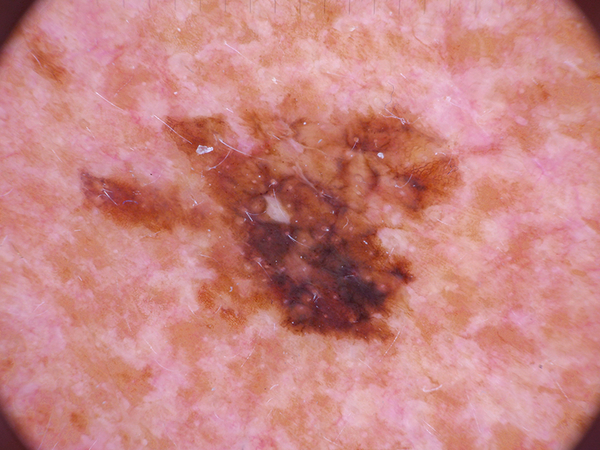
\includegraphics[width=\textwidth]{./images/ISIC_0024310.jpg}
            \caption{Image with black frame}
        \end{subfigure}
        \begin{subfigure}[b]{0.3\textwidth}
            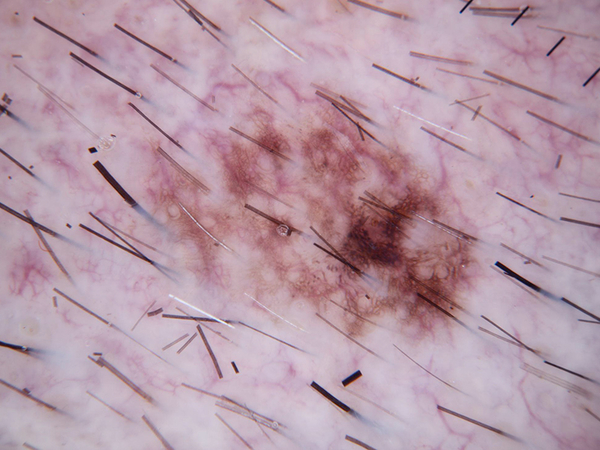
\includegraphics[width=\textwidth]{./images/ISIC_0024420.jpg}
            \caption{Image with ruler}
        \end{subfigure}
        \begin{subfigure}[b]{0.3\textwidth}
            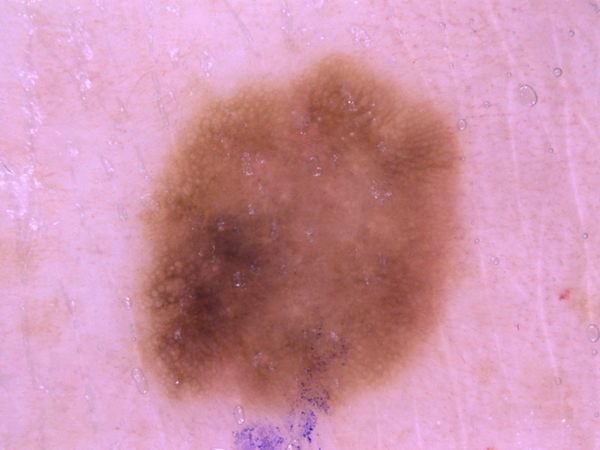
\includegraphics[width=\textwidth]{./images/ISIC_0027514.jpg}
            \caption{Image with blue ink}
        \end{subfigure}
    \end{center}
    \caption{Images with different confounding objects}
    \label{fig:confounding_objects}
\end{figure}

Labeling some of these confounding objects, we see that the rulers occur way more often than the others with a prevalence of roughly $17\%$ (See Table \ref{table:confounding_objects}).
Due to this higher prevalence, the study done in this project will focus on the ruler markings over the other confounding objects.

\begin{table}
    \centering
    \begin{tabular}{|l|r|}
        % confounding_objects.ipynb
        \hline 
        Confounder &  Prevalence \\ \hline
        ruler   &  0.171842 \\ \hline
        sticker &  0.000100 \\ \hline
        ink     &  0.003495 \\ \hline
    \end{tabular}
    \caption{Dataset prevalence of confounding objects}
    \label{table:confounding_objects}
\end{table}


\pagebreak

\section{Theory}
This report assumes that the reader is familiar with the basics of machine learning.
This includes basic linear algebra, data preprocessing and model selection.
Further a basic understanding of how neural networks function is assumed,
including the basic concept of gradiant descent used for model training.


\subsection{Tensors}
The following definitions and concepts are heavily based on \textit{Introduction to Convolutional Neural Networks} by J. Wu \cite{tensorIntroduction}.
In linear algebra, the concept of a vector is introduced.
Further a 2-dimensional vector is introduced, the \textit{matrix}.
We will denote a vector as $\vecsym{v}\in \mathbb{F}^n$ and a matrix as $\matsym{M}\in \mathbb{F}^{m\times n}$.
Here $\mathbb{F}$ is a field.
For the purpose of this report, a field can be considered a set of element with a defined addition and multiplication operation.
Especially most of the time the field will be the real numbers, $\mathbb{R}$.

Having defined vectors and matrices, we can now define a tensor as the natural extension of the matrix abstraction,
by adding more dimensions.
A $3$-dimensional tensor is can then be defined as $\tenssym{T}\in \mathbb{F}^{m\times n\times c}$.
Such a tensor is a natural way to represent an image in colors.
Such a representation of an image of height $h$ and width $w$ could then be represented as an
element in $\mathbb{F}^{h\times w\times 3}$.

An example of a higher order tensor used in this project, could be a batch of images.
Such a batch could be represented as a tensor of shape $(h, w, c, b)$ where $b$ is the batch size. 
That is, the entire batch would be a $4$-dimensional tensor in the tensor-space $\mathbb{F}^{h\times w\times c\times b}$.

\paragraph{Vectorizing tensors}
As noted in most introductions of linear algebra, matrices are themselves vectors.
This is to be understood as, any matrix $\matsym{M} \in \mathbb{F}^{m\times n}$ can be represented as a vector $\vecsym{m} \in \mathbb{F}^{m\cdot n}$.
This is commonly done by stacing the columns of the matrix, e.g.  if 
\begin{equation}
\matsym{M} = \begin{bmatrix}
    m_1 & m_2 & m_3 \\
    m_4 & m_5 & m_6 \\
    m_7 & m_8 & m_9
\end{bmatrix} \in \mathbb{F}^{3 \times 3}
\end{equation}
then the vector representation is
\begin{equation}
\vecsym{m} = \begin{bmatrix}
    m_1 & m_4 & m_7 & m_2 & m_5 & m_8 & m_3 & m_6 & m_9
\end{bmatrix}^T \in \mathbb{F}^{9}
\end{equation}
The same concept can be applied to tensors of higher dimensions than the $2$-dimensional matrix,
by stacking the columns continously.

\paragraph{Partial derivatives over vectors} \label{sec:partial_derivatives_of_scalar_over_vector}
In multiple setings in training of neural networks, it is neccesarry to figure out what
parts of the model contributed to the result of the model.
During training, we for instance want to know what parts of the model contributed to an increase of the loss function,
so that these parts can be changed thereby hopefully improving the model.
In this report it is also used for creating saliency maps, and discussing them (see section \ref{sec:gradiant_saliency_maps}).

Defining the partial derivative of a vector $\vecsym{v}\in\mathbb{F}^n$ with respect to a scalar $s$ is done as follows:
\begin{equation}
    \left[ \frac{\partial s}{\partial \vecsym{v}} \right] = \frac{\partial s}{\partial \vecsym{v}_i}
\end{equation}

Note that with this definition, derivatives over matrices can also be done by first vectorizing them,
and we then get the nice algebraic property that  $\frac{\partial s}{\partial \vecsym{v}}^{T} = \frac{\partial s}{\partial \vecsym{v}^{T}}$ 


\paragraph{Partially deriving vector functions}
Suppose $\vecsym{x} \in \mathbb{F}^n$, 
$f: \mathbb{F}^n \rightarrow \mathbb{F}^m$ and
$\vecsym{y} = f(\vecsym{x}) \in \mathbb{F}^m$.
Then
\begin{equation}
    \left[ \frac{\partial \vecsym{y}}{\partial \vecsym{x}^T} \right]_{ij} =
    \frac{\partial \vecsym{y}_i}{\partial \vecsym{x}_j}
\end{equation}

Which means that the derivative of a vector function on the form of $f$ will be a matrix/$2$-tensor
in the tensor-space $\mathbb{F}^{m\times n}$.


\subsection{Convolutional neural networks (CCNs)} \label{sec:convolutional_neural_networks}
Convolutional neural networks (CNNs) are a fairly modern method used in image classification.
They are based on the idea of a convolutional layer, which is a way of combining pixels in a
neighbourhood of an image into single features.

The mathemathical basis is the \textit{convolution} of a matrix.
During the definition of convolutions, the following matrix will be used as an example:
\begin{equation}
    \matsym{I} = \input{build/convolution_example/I.tex}
\end{equation}

Think of $\matsym{I}$ as an image.
Sematically there is an area in the \"image\" that has way higher values than the rest
(the lower right corner).
A convolution on the image, will reduce this information to a more compact representation.
To do this, a matrix kernel needs to be defined. It's standard to use a square kernel.
Here we will use a $3 \times 3$ kernel:
\begin{equation}
    \matsym{K} = 
        \input{build/convolution_example/K.tex}
\end{equation}

To then convolve $\matsym{I}$ with $\matsym{K}$, we \textit{move} the kernel over the image,
and multiply each index of the kernel with the index that it is currently \textit{above} in the image
(a full mathemathical deifintion follows lates in section \ref{sec:convolution_definition}).
That will in this case result in the matrix:
\begin{equation}
    \input{build/convolution_example/convolution.tex}
\end{equation}


On Figure \ref{fig:convolution_example} heatmaps of the original $I$ and the convolved, shows that they look very similar.
\begin{figure}[h]
\centering
\begin{subfigure}{0.45\textwidth}
    \includegraphics[width=\textwidth]{build/convolution_example/I.png}
    \caption{Original version of $I$}
\end{subfigure}
\begin{subfigure}{0.45\textwidth}
    \includegraphics[width=\textwidth]{build/convolution_example/convolution.png}
    \caption{Convolution of $I$ with $K$}
\end{subfigure}
\caption{Heatmaps of the original $I$ and the convolved $I$}
\label{fig:convolution_example}
\end{figure}

Comparing the heatmaps on Figure \ref{fig:convolution_example}, makes it clear that little to no imformation about
where the high values are in the picture has been lost.
The amount of data points has however been reduced.

\paragraph{Padding}
The current model of moving the kernel over the image, will not prioritize the borders
of the image a lot. 
To compat this, the image is often padded - usually with zeros. 
This is done by adding a border of zeros around the image, the width of which is refered to as the size of the padding.
By default, the padding in libaries like PyTorch \cite{PyTorch} is $0$ (no padding) as in the example before.

To continue the example, we will now use a padding of $1$ around the image.
\begin{equation}
    \matsym{I}_{\text{padded}} = \input{build/convolution_example/I_padded.tex}
\end{equation}

Calculating the convolution of the padded image with the kernel, results in the following matrix:
\begin{equation}
    \input{build/convolution_example/convolution_padded.tex}
\end{equation}

And again plotting the heatmaps we see two similar images again:
\begin{figure}[h]
\centering
\begin{subfigure}{0.45\textwidth}
    \includegraphics[width=\textwidth]{build/convolution_example/I.png}
    \caption{The original $\matsym{I}$}
\end{subfigure}
\begin{subfigure}{0.45\textwidth}
    \includegraphics[width=\textwidth]{build/convolution_example/convolution_padded.png}
    \caption{Convolution of $\matsym{I}_{\text{padded}}$ with $K$}
\end{subfigure}
\caption{Heatmaps of the padded $\matsym{I}_{\text{padded}}$ and the convolved $\matsym{I}_{\text{padded}}$}
\label{fig:convolution_example_padded}
\end{figure}

Note that padding increases the amount of data points in the image, but that
the effect of this is not as extreme as it seems in the example, since images a usually
a lot larger than this small example.

\paragraph{Stride}
To reduce the amount of data points even further, we can use a stride.
This is done by moving the kernel over the image as before, but moving multiple pixelse each time.

Following the example from before using a stride of $2$ and a padding of $1$, the convolution results in the following matrix:
\begin{equation}
    \input{build/convolution_example/convolution_stride.tex}
\end{equation}

This is again plotted in Figure \ref{fig:convolution_example_stride}.

\begin{figure}[ht]
\centering
\begin{subfigure}{0.45\textwidth}
    \includegraphics[width=\textwidth]{build/convolution_example/I.png}
    \caption{The original $\matsym{I}$}
\end{subfigure}
\begin{subfigure}{0.45\textwidth}
    \includegraphics[width=\textwidth]{build/convolution_example/convolution_stride.png}
    \caption{Convolution of $\matsym{I}_{\text{padded}}$ with stride $2$}
\end{subfigure}
\caption{Heatmaps of the original $\matsym{I}$ and the convolved $\matsym{I}_{\text{padded}}$}
\label{fig:convolution_example_stride}
\end{figure}

It is again clear that the data seems similar to the original image, but the data points
has been reduced from $\input{build/convolution_example/I_size.tex}$ to $\input{build/convolution_example/final_convolution_size.tex}$.

In convolutions can combine information from data where some kind of \textit{proximity} is important.
This is very much the case in image analysis (hence the focus in this explanation), but the idea is
not limited to this field.

\paragraph{Full definition of convolutions}\label{sec:convolution_definition}
The above is a very simple example of a convolution.
A full compact formula for making a convolution is left out, as it is not readable and
ultimately not very insightful. 
Instead we will make a implementation of the a \verb|convolve| function in Python.
To define such an algorithm, it is usefull to know the output size of the final matrix.
Let the width of the original image be $w$, the kernel size be $k$, the padding be $p$, and the stride be $s$.
Calculating the output width can then be done by finding all the possible values of $w$ that can be
used as the left value of the kernel.
First the padded size of the image is seen to be $w + 2p$.
Since a kernel is moved over the picture, the last $k-1$ pixels cant be used to place a kernel.
Assuming that the image is non-empty and the kernel is smaller than or the same size as the image,
at least one kernel can be placed, adding up to a total of $k$ pixels where a kernel cannot be placed.
Of the remaining only $1/s$ of the pixels are actually used to place a kernel, hence the output width becomes:
\begin{equation}
    w_{out} = \left\lfloor \frac{w + 2p - k}{s}\right\rfloor + 1
\end{equation}

And with a completely similar procedure for the height, $h$, we get:
\begin{equation}
    h_{out} = \left\lfloor \frac{h + 2p - k}{s} \right\rfloor + 1
\end{equation}

Having these values, we can then define a Python function that performs the convolution:

\inputminted[]{python}{src/convolve.py}

\subsection{The power of convolution kernels}
In the example in Section \ref{sec:convolutional_neural_networks}, a convolution that
comprimed the image into a condensed version was used.

Kernels can do lot more than compressing images though.
For the following, different types of kernels are used to convolute an image of a Model of the Greek Temple of Artemis \cite{greek-temple-picture}.

With a kernel like this:
\begin{equation}
    K_{\text{edge}} = \input{build/kernel_examples/K_edge.txt} 
\end{equation}
an image is produced where the edges are highlighted.

\begin{figure}[ht]
\centering
\begin{subfigure}{0.45\textwidth}
    \includegraphics[width=\textwidth]{build/kernel_examples/image_scaled.jpg}
    \caption{The original image}
\end{subfigure}
\begin{subfigure}{0.45\textwidth}
    \includegraphics[width=\textwidth]{build/kernel_examples/edges.jpg}
    \caption{The image considered as a matrix convolved with $K_{\text{edge}}$}
\end{subfigure}
\caption{The image with the edges highlighted}
\end{figure}

In a similar way, a kernel like this:
\begin{equation}
    K_{\text{vertical}} = \input{build/kernel_examples/K_vertical.txt}
\end{equation}
can be used to highlight the vertical lines in the image.

\begin{figure}[ht]
\centering
\begin{subfigure}{0.45\textwidth}
    \includegraphics[width=\textwidth]{build/kernel_examples/image_scaled.jpg}
    \caption{The original image}
\end{subfigure}
\begin{subfigure}{0.45\textwidth}
    \includegraphics[width=\textwidth]{build/kernel_examples/vertical.jpg}
    \caption{The image considered as a matrix convolved with $K_{\text{vertical}}$}
\end{subfigure}
\caption{The image with the vertical lines highlighted}
\end{figure}

A lot of other interesting kernels exist, see for instance these examples at AI Shack \cite{kernel-example-webpage}.

The point we want to make here, is that a lot of different information can be extracted from an image,
if the correct kernel is used.
When training a convolutional layer of a neural network, it is exactly the kernel values that optimized.

\subsection{Gradients of neural networks}


\subsection{Backpropagation}

\subsection{The Resnet architecture}

\subsection{Saliency maps}

\paragraph{Gradiant based saliency maps} \label{sec:gradiant_saliency_maps}

\pagebreak


\printbibliography[title={Litterature}]
\end{document}